\documentclass[output=paper]{langsci/langscibook}

\author{Pegah Faghiri\affiliation{Universiteit van Amsterdam} \lastand Pollet   Samvelian\affiliation{Université Sorbonne Nouvelle}}


\title{The issue of ``separability'' in Persian complex predicates}

\abstract{This paper addresses the issue of separability in Persian complex predicates (CPs). These are syntactic combinations formed by a verb and a preverbal element (noun, adjective, preposition) realizing a single conceptual unit. Although the separability of the components of a CP by morphological and grammaticalized elements (e.g. auxiliaries) is not a matter of controversy, the possibility for ``real'' syntactic constituents to interrupt a CP continues to be debated.
Building on an experimental study, we show that real syntactic material can separate the components of a CP and suggest that this separability can be viewed as a word order variation phenomenon, comparable to the one observed for direct objects (DO) and indirect objects (IO) in the preverbal domain.
The semantic bond nevertheless plays a role in granting CPs some hallmarks of ``wordhood'', favoring their adjacency, among other things.}


\begin{document}
\maketitle

\section{Introduction}

\begin{sloppypar}
  In this paper, we address the issue of separability in Persian
  complex predicates (CPs). Building on an experimental study, we show
  that real syntactic material can separate the components of a CP, a
  possibility generally underestimated or denied in most previous
  studies on Persian CPs. We also suggest that this separability can
  be viewed as a word order variation phenomenon, comparable to the
  one observed for direct objects (DO) and indirect objects (IO) in
  the preverbal domain. As such, it is best accounted for by soft
  constraints on word order, that is, (statistical) preferences,
  involving a set of functional factors, rather than by categoric
  syntactic, or phrase structure, rules (hard constraints). Likewise,
  we do not consider that the strong preference for the components of
  the CP to occur adjacent to each other is peculiar to CPs, hence
  requiring a specific syntactic treatment. This preference is also
  observed for bare objects in Persian, which tend to occur adjacent
  to the verb. The fact that it becomes even stronger in the case of
  CPs is completely expected, given that semantic relatedness favors
  adjacency.  Thus, on the one hand, the fact that several words form
  a single conceptual unit favors their remaining together (one
  semantic unit), while on the other hand, the fact that the sequence
  is made up of multiple syntactic units still allows for the word
  order preference rules to apply.
\end{sloppypar}

It is a well-known fact that the verbal lexicon in Persian is overwhelmingly formed by complex predicates, that is, multiword expressions including a verb and a non-verbal element, mainly a noun, such as \textit{b\=azi kardan} `to play' (play do) or \textit{qadam zadan} `to walk' (step hit), also known as ``light verb constructions'' (LVCs).\footnote{There are also CPs formed with an adjective, e.g. \textit{b\=az kardan} `to open' (open do), a preposition or particle, e.g. \textit{bar d\=a\v{s}tan} `to take' (\textsc{PART} have) or a prepositional phrase \textit{be k\=ar bordan} `to use' (to work take). In this paper, we will focus on noun-verb CPs.}

Forming one semantic unit, the components of a CP tend to remain together and resist separation, except by morphological or grammaticalized material (verbal prefixes, clitic pronouns, auxiliaries). This has led many researchers to take a strong stance on this issue, claiming that “real” syntactic material can never intervene between the verb and the non-verbal unit of a CP. This claim has served as a key argument in favor of the ``wordhood'' \citep[][134--135]{Goldberg1996} or a ``lexical analysis'' \citep{dabir1997compound,Karimi-Doostan1997} of CPs, along with other properties, which are typical of words, or rather, lexemes in this case. Namely:

\begin{itemize}
	\item The whole sequence generally has a conventional meaning that must be learned by the speakers. In other words, it is idiomatic, in that the meaning associated with the sequence cannot be fully derived from its components' meaning \citep{Goldberg1996,Karimi-Doostan1997,Samvelian2001,Samvelian2012,SamFag2013}. 
	\item
          \begin{sloppypar}
            It can serve as input to morphological word formation
            rules that derive new lexemes from existing ones
            \citep{Goldberg1996,Karimi-Doostan1997,Megerdoomian2002,Vahedi-Langrudi:1996}.
          \end{sloppypar}
\end{itemize}

The supposed inseparability of the CP components has further been used to draw a clear-cut distinction between the latter on the one hand and ordinary verb-complement syntactic combinations on the other hand, and to support a specific syntactic analysis of CPs, which distinguishes them from ordinary syntactic combinations involving a verb and its object \citep[with the notable exception of][]{Muller2010,Samvelian2001,Samvelian2012,SamFag2014,SamFagBLS}.

Although \citet[][55--87]{Samvelian2012} extensively discusses this issue and provides several attested examples showing that almost all CPs can undergo separation, the controversy seems to still persist since more recent studies \citep[e.g.][]{SafaviEtal2016} take the inseparability of at least some classes of CPs as empirically uncontroversial.


In this paper, we will first present the basic empirical facts about Persian CPs and their syntactic properties as they have been discussed in the literature, with a special focus on the issue of separability. In particular, we will examine Karimi-Doostan's claim about the relationship between the separability and the predicative nature of the nominal element in noun-verb CPs. Contra Karimi-Doostan, we will provide experimental evidence showing that the nominal element of a CP, regardless of its type and its degree of determination, can be separated from the verb by syntactic material. 

Comparing the results of our experiments with the findings of some recent studies on word order variations in the preverbal domain in Persian \citep{FaghiriPhd,FagSam2014,FagSamHem2018}, which also resort to quantitative methods, we will argue that noun-verb CPs, on the whole, behave in the same way as DO-verb combinations with respect to word order preferences. Crucially, the latter involve preferences rather than strict syntactic constraints. 


It has been shown that different (functional) factors (e.g.~givenness, animacy, length) interact to determine the linear order of constituents, when the latter is not constrained by the grammar. Some of these factors (degree of determination, heaviness and animacy) have also been shown to intervene in ordering preferences regarding direct and indirect objects in Persian as well \citep{FaghiriPhd}. We will see that the same factors are at play in determining the ordering preferences of CPs components. Furthermore, semantic relatedness and collocational relation are two factors known to favor adjacency \citep[see e.g.][]{hawkins2001,wasow2002}. Hence, the tendency for the components of a CP to appear adjacent is not surprising, since they convey one conceptual meaning. 

\section{Existing claims on the inseparability of CPs}\label{Sec:Claims}

Several studies on Persian CPs claim that the separability of the components of a CP is subject to significant restrictions. According to \citet{Goldberg1996}, only morphological and ``grammatical'' material may intervene between the non-verbal element and the verb, as illustrated in (\ref{sep-morpho}).

\begin{exe}
	\ex \label{sep-morpho}
	\begin{xlist}
		\ex[]{\gll omid goli=r\=a set\=aye\v{s} ne-mi-konad\\
			Omid  Goli=\gloss{ra} praise \gloss{neg-ipfv}-do.prs-\gloss{3sg}\\
			\glt `Omid doesn't praise Goli.'\label{sep-morpho-aff}}
		\ex[]{\gll omid set\=aye\v{s}=a\v{s} kard\\
			Omid  praise=\gloss{cl.3sg} did.\gloss{pst}\\
			\glt `Omid praised her/him.'\label{sep-morpho-cl}}
		\ex[]{\gll omid set\=aye\v{s}=a\v{s} x\=ahad kard\\
			Omid  praise=\gloss{cl.3sg} \gloss{aux.fut.3sg} do.\gloss{sinf}\\ 
			\glt `Omid will praise her/him.'\label{sep-morpho-aux}}
	\end{xlist}
\end{exe}


In (\ref{sep-morpho-aff}), the nominal element of the CP \textit{set\=aye\v{s} kardan} `to praise' (praise do), namely \textit{set\=aye\v{s}} `praise', is separated from the verb by the negation prefix \textit{na}- and the aspect-mode prefix \textit{mi}-. In (\ref{sep-morpho-cl}), the clitic pronoun =\textit{a\v{s}}, which refers to the direct object in the first example, attaches to the nominal element and thus separates it from the verb. Finally, in (\ref{sep-morpho-aux}), the intervening element is the tense auxiliary \textit{x\=astan} `to want', which is an independent word. 

\citet{Goldberg1996} claims that ``real'' syntactic material, on the other hand, cannot occur between the components of the CP. This restriction is illustrated by the examples in (\ref{goldberg-adv}), adapted from \citet[134--135]{Goldberg1996}: 


\begin{exe}
    \judgewidth{??}
	\ex\label{goldberg-adv}
	\begin{xlist}
		\ex[]{\gll tond r\=anandegi kard-am\\
			quickly driving  do.\gloss{pst-1sg}\\
			\glt `I drove quickly.'\label{goldberg-adv-a}		}
		\ex[??] {\gll r\=anandegi tond kard-am\\
			driving quickly do.\gloss{pst-1sg}\\
			\glt (Intended) `I drove quickly.'\label{goldberg-adv-b}}
	\end{xlist}
	
	\ex\label{goldberg-sep-do}
	\begin{xlist}
		\ex[]{\gll  ali=r\=a set\=aye\v{s} kard-am\\
			Ali=\gloss{ra} praise do.\gloss{pst-1sg}\\
			\glt `I adored Ali.'\label{gold-sep-do-1}}
		\ex[??]{\gll set\=aye\v{s} ali=r\=a kard-am\\
			praise  Ali=\gloss{ra}  do.\gloss{pst-1sg}\\
			\glt (Intended) `I adored Ali.'\label{gold-sep-do-2} (Goldberg 1996, p.~135, e.g.~3)}	
	\end{xlist}
\end{exe}



According to \citet{Goldberg1996}, (\ref{goldberg-adv}b) shows that the placement of a modifier adverb such as  \textit{tond} `quickly' between the nominal element and the verb makes the sentence odd. The adverb must precede the whole CP, as in (\ref{goldberg-adv}a), while, in ordinary object-verb combinations, a modifier adverb can intervene between the object and the verb, as shown by (\ref{goldberg-sep-do2}). Example (\ref{goldberg-sep-do}b) shows that the direct object cannot interrupt the CP and must be placed before it, as in (\ref{goldberg-sep-do}a). 

\begin{exe}
	\ex\label{goldberg-sep-do2}
	\gll ma\v{s}q=am=r\=a tond neve\v{s}t-am\\
	homework=\gloss{cl.1sg}=\gloss{ra} quickly write.\gloss{pst-1sg}\\
	\glt `I did my homework quickly.'(Goldberg 1996, p.~134, e.g.~10)
\end{exe}

These facts,  \citet{Goldberg1996} argues, imply that CPs are single syntactically integrated predicates, comparable to some extent to words (or lexical units). As such, they are subject to constraints which do not apply for ordinary syntactic combinations. These constraints may nevertheless be violated in some contexts, allowing for morphological (affixes and clitics) and grammatical elements (auxiliaries)  to intervene between the components of a CP.


Contrary to \citet{Goldberg1996}, Karimi-Doostan (\citeyear{Karimi-Doostan1997}, \citeyear{Karimi-Doostan:2011}) admits that the components of a CP can be separated by syntactic elements depending on the type of the nominal element of the CP. The latter are classified into three categories: predicative nouns, e.g. \textit{latme} `damage', verbal nouns, e.g. \textit{ers\=al} `sending',  and non-predicative nouns, e.g. \textit{gu\v{s}} `ear'. It is claimed that only CPs formed by predicative nouns are separable. 
The rationale  is that for the nominal element to be separable from the verb, it needs to meet the following two conditions (in the context of a given CP): 

\begin{enumerate}\label{claim}
	\item It must have an argument structure.
	\item It must be able to project a DP/NP, that is, be determined or quantified.
	
\end{enumerate}

Only predicative nouns, it is claimed, can fit these conditions, as illustrated by examples (\ref{kd-latme})--(\ref{kd-gush}). 

\begin{exe}
	\ex\label{kd-latme}
	\begin{xlist}
		\ex[]{\gll latme=ye tagarg be b\=aq=e man  \\
			damage=\gloss{ez} hail   to garden=\gloss{ez} \textsc{1.sg}\\
			\glt `hail damage to my garden'
		}
		\ex[]{\gll tagarg be b\=aq=e man latme zad\\
			hail   to garden=\gloss{ez} \textsc{1.sg} damage hit.\gloss{pst.3sg}\\
			\glt `The hail damaged my garden.'\label{kd-latme-bare}
		}
		\ex[]{\gll tagarg latme=ye bad=i be b\=aq=e man zad\\
			hail   damage=\gloss{ez} bad=\gloss{indf} to garden=\gloss{ez} \textsc{1.sg} hit.\gloss{pst.3sg}\\
			\glt `The hail damaged my garden badly.'\label{kd-latme-ind}
		}
	\end{xlist}

	\ex\label{kd-anjm}
	\begin{xlist}
		\ex[]{\gll anj\=am-e k\=ar tavassot=e ali\\
			performing=\gloss{ez} work by=\gloss{ez} Ali\\
			\glt	`Ali's doing the work'
		}
		
		\ex[]{\gll ali k\=ar=r\=a anj\=am   d\=ad\\
			Ali work=\gloss{ra} performing give.\gloss{pst.3sg}\\
			\glt   `Ali did the work.'
		}
		
		\ex[*]{\gll ali anj\=am-e xub=i be k\=ar  d\=ad\\
			Ali performing=\gloss{ez} good=\gloss{indf} to work  give.\gloss{pst.3sg}\\
			\glt	(Intended) `Ali did the work well.'
		}
	\end{xlist}

	\ex\label{kd-gush}
	\begin{xlist}
		
		\ex[*]{\gll gu\v{s}=e ali be r\=adyo\\
			ear=\gloss{ez} Ali to radio \\
			\glt	(Intended) `Ali's listening to the radio'
		}
		
		
		\ex[]{\gll ali be r\=adyo gu\v{s} d\=ad\\
			Ali to radio ear give.\gloss{pst.3sg}\\
			\glt	`Ali listened to the radio.'
		}
		
		
		\ex[*]{\gll ali gu\v{s}-e xub=i be r\=adyo  d\=ad\\
			Ali ear=\gloss{ez} good=\gloss{indf} to radio  give.\gloss{pst.3sg}\\
			\glt	(Intended) `Ali listened to the radio well.'\label{kd-gush-ind}
		}
		
	\end{xlist}
\end{exe}


\textit{Latme} `damage', e.g. (\ref{kd-latme}), is a predicative noun. It has an argument structure, as shown by its ability to realize its arguments within an DP/NP, e.g. (\ref{kd-latme}a). As the nominal element of the CP \textit{latme zadan} `to damage', \textit{latme} must be adjacent to the verb when it is realized as a bare noun, e.g. (\ref{kd-latme}b). When determined, the nominal element of the CP functions as the nominal argument of the verb. It becomes autonomous and can be separated from the verb by various syntactic constituents. This is illustrated by (\ref{kd-latme}c),  where \textit{latme} `damage' carries the indefinite determiner, the enclitic =\textit{i}, and consequently can precede the prepositional argument.



Like predicative nouns, verbal nouns, e.g. \textit{ers\=al} `sending' and \textit{anj\=am} `doing, accomplishment', also carry an argument structure, e.g. (\ref{kd-anjm}a). However, unlike the former, they cannot project a DP/NP, since they have limited nominal behavior: they cannot be pluralized, modified, quantified and determined.  
These nouns are broadly assumed to form prototypical light verb constructions, e.g. \textit{ers\=al kardan} `to send', \textit{anj\=am d\=adan} `to accomplish, to do'. In this case, they always occur in their bare form and hence adjacent to the verb, e.g. (\ref{kd-anjm}b). These properties of verbal nouns explain the ungrammaticality of (\ref{kd-anjm}c).

Finally, non-predicative nouns, e.g. \textit{gu\v{s}} `ear', do not carry argument structure, as illustrated by (\ref{kd-gush}a). When used outside a CP, these nouns can develop into DP/NPs, e.g. \textit{in gu\v{s}} `this ear'. However, when used as the nominal element of a CP, e.g. \textit{gu\v{s} kardan} `to listen', they can only appear in their bare form, e.g. (\ref{kd-gush}b), and therefore must remain adjacent to the verb, hence the ungrammaticality of (\ref{kd-gush}c).


\section{Severing separability from DP/NP projection}\label{Sec:Severing}

Before investigating the separability of the components of a CP, it should be made clear that Karimi-Doostan's claims involve two different, though perhaps interrelated, issues:

\begin{enumerate}\label{claim-2}
	\item The first issue concerns the possibility for the bare nominal element of the CP to be separated from the verb by syntactic material. 
	\item
          \begin{sloppypar}
            The second issue is the possibility for the nominal
            element of the CP to project a DP/NP and thus to behave as
            an autonomous syntactic constituent with respect to the
            verb.
          \end{sloppypar}

\end{enumerate}

Under Karimi-Doostan's view, these two issues are entangled since separation is possible only for DP/NPs. However, several studies on Persian CPs provide examples of bare nominal elements of CPs which are not adjacent to the verb:


\begin{exe}
	\ex\label{ct}
	\begin{xlist}		
		\ex[]{\gll ... va   sili   be surat=am   zad\\
			{} and slap to face=\gloss{cl.1sg}   hit.\gloss{pst.3sg}\\
			\glt `...and (s)he slapped me (on the face).'\footnote{This is an attested example taken from the novel \textit{Souva\v{s}un} by S. Dane\v{s}var \citep{Samvelian2012}.}\label{ct-sili} 		\hfill \citep[][p.~40, ex.~29]{Samvelian2012}}
		
		\ex[]{\gll  gu\v{s} be man ne-mi-kon-e\\
			ear to \textsc{1.sg} \gloss{neg-ipfv}-do-\gloss{3sg}\\
			\glt `(S)he doesn't listen to me.'\label{ct-gush} 	\hfill \citep[p.~197, ex.~7]{MohammadKarimi1992}}
		
		\ex[]{\gll  kimi\=a in ot\=aq=r\=a extes\=as be mehm\=an d\=ad\\
			Kimea this room=\gloss{ra} allocation to guest give.\gloss{pst.3sg}\\
			\glt `Kimea allocated this room to the guest.'\label{ct-extesas} 	\hfill \citep[p.~199, ex.~16]{MohammadKarimi1992}	}		
		
	\end{xlist}
\end{exe}

In (\ref{ct}a), the predicative noun \textit{sili} `slap', which occurs as a bare noun, is nevertheless separated from the verb by the PP argument of the CP. In (\ref{ct}b), the PP argument intervenes between the non-predictive noun  \textit{gu\v{s}} `ear',  again in its bare form, and the verb. (\ref{ct}c) illustrates the possibility for a verbal noun to precede the PP argument.\footnote{\citet{Samvelian2012} provides numerous similar examples attested in contemporary Persian literature and websites. For more attested examples see also the PersPred Database http://www.perspred.cnrs.fr.}

These examples show that the possibility for bare nominal elements of CPs to be separated from the verb is a matter of controversy. Contra \citet{Goldberg1996} and \citet{Karimi-Doostan1997,Karimi-Doostan:2011}, \citet{Samvelian2012} claims that the adjacency of the bare nominal element and the verb in a CP is a matter of strong preference and not a strict constraint. She further draws a parallel between these bare nominal elements and bare objects of lexical verbs, which also tend to occur adjacent to the verb, as it has been noted in all studies on the syntax of Persian \citep[][among many others]{dabir1997compound,givi,ghomeshi1996phd,lazard82,mahootian97,Samvelian2001,Karimi2003}. 
Like bare objects, bare nominal elements of CPs can nevertheless be separated from the verb by syntactic material. Their greater reluctance to separation, compared to bare objects of lexical verbs, is due to the idiomatic relation between the components of a CP and their closer semantic relatedness, which favors even more adjacency. 

To sum up, one issue to be addressed when talking about the separability of CP components is whether the bare nominal element can be separated from the verb by real syntactic material, and, if so, what are the parameters that favor this possibility. 

Another issue is the possibility for the nominal element of the CP to project a DP/NP, regardless of its being adjacent to the verb. Recall that according to Karimi-Doostan, only predicative nouns display this property. In particular, concrete nouns like \textit{gu\v{s}} `ear' are claimed to always occur in their bare form when part of a CP.

Here again, several counterexamples can be found in the literature, where a concrete noun participating in a CP is nevertheless determined, quantified or modified:

\begin{exe}
	\ex\label{samvelian-concrete}
	\gll t\=a \v{c}\=ay xonak \v{s}av-ad u sar=i be mahhal=e serqat zad \\
	until tea cool become.\gloss{sbj-3sg} he head=\gloss{indf}  to place=\gloss{ez} burglary hit.\gloss{pst.3s}\\
	\glt `Until his tea cools, he went to visit the place the burglary had taken place.'\footnote{Attested example from \textit{Zan-e zi\=adi} by J. Al Ahmad (short stories).} 	\hfill \citep[][p.~85, ex.~68]{Samvelian2012}
\end{exe}


In this attested example from a contemporary Persian novel, the nominal element of the CP \textit{sar zadan} `to visit' (lit. `head hit') projects a DP/NP \textit{sar=i} `a head', since it is determined by the indefinite determiner =\textit{i}. This example and many others mentioned in \citet{Samvelian2012} show that not all concrete nouns are incapable of projecting a DP/NP in the context of a CP. The question, as for the previous case, is whether the possibility for a noun to project a DP/NP in the context of a given CP can be correlated with some of its properties.

In this paper, we will focus on the first issue, that is, the separability of the nominal element of the CP. Since the nominal element of the CP is to some extent comparable to a bare direct object, we will compare the possibility for these two elements to be non-adjacent to the verb. Our purpose is to check to what extent the constraint or the preference for the bare nominal element to be adjacent to the verb parallels the tendency for bare DOs to  precede the verb immediately. To put it differently, up to now, the issue of  separability of the components of a CP has generally been investigated without considering the wider issue of ordering preferences in Persian, especially those involving direct and indirect objects. This is surprising since the literature on Differential Object Marking (DOM) in Persian has extensively discussed the tendency for bare direct objects to be adjacent to the verb, contrary to marked objects, which undergo scrambling. 

In the next section, we will present basic word order properties of sentences involving a direct and an indirect object in Persian, with a special focus on recent findings from a series of corpus and experimental studies \citep{FaghiriPhd,FagSam2014,FagSamHem2014,FagSamHem2018}.



\section{Bare objects and their position in Persian}\label{Sec:WO}

The unmarked (neutral or canonical) word order in Persian is SOV. In ditransitive constructions, the ordering of the direct and the indirect object has been claimed to be dependent on the markedness of the direct object: unmarked DOs follow the IO and occur adjacent to the verb, (\ref{do-io}a), while marked DOs precede the IO, (\ref{do-io}b), and consequently, are separated from the verb \citep[][among many others]{Browning&Karimi,mahootian97,Karimi2003}. 
Persian displays DOM. As illustrated in (\ref{do-io}b), definite and/or specific DOs are marked by the enclitic =\textit{r\=a}, which attaches to the last word of the DO. Note also that in formal Persian, there is no overt marker for definiteness, as shown by the fact that \textit{gol} `flower' has the same form in (\ref{do-io}a) and (\ref{do-io}b), albeit two different readings with respect to determination.\footnote{For DOs, the ambiguity is resolved due to the presence of =\textit{r\=a}. Bare subjects, by contrast, are ambiguous between an existential or a kind-level generic reading and a definite/specific reading. Thus, in a sentence like \textit{gol ru-ye miz bud}, two readings are available for \textit{gol}: `A flower/flowers were on the table' or `The flower was on the table'.}

It should also be noted that in Persian, bare nouns,\footnote{Note that we use the label ``bare'' here to refer to nouns that not only appear in their bare form, but also have a non-determined and non-quantified reading. This means that in (\ref{do-io}b), \textit{gol} `flower' is not considered as a bare noun since it receives a definite reading.} that is, nouns without any determination or quantification like \textit{gol} in (\ref{do-io}a), are not specified for number and therefore can yield a mass reading. Bare objects have either an existential, as in (\ref{do-io}a), or a kind-level/generic reading, as in (\ref{bare-kind}).

\begin{exe}
	\ex\label{do-io}
	\begin{xlist}
		
		\ex[]{\gll maryam be s\=ar\=a gol d\=ad\\
			Maryam to Sarah  flower give.\gloss{pst.3sg}\\
			\glt `Maryam gave a flower/flowers to Sarah.'\label{do-bare}
		}
		
		\ex[]{\gll maryam gol=r\=a be s\=ar\=a  d\=ad\\
			Maryam flower=\gloss{ra} to Sarah give.\gloss{pst.3sg}\\
			\glt `Maryam gave the flower to Sarah.'\label{do-ra} 
		}
		
	\end{xlist}
	
	\ex\label{bare-kind}
	\gll maryam gol dust d\=ar-ad\\
	Maryam flower friend have.\gloss{prs.3sg}\\
	\glt `Maryam likes flowers.'
\end{exe}

Indefiniteness, on the other hand, is overtly marked in Persian. It can be realized by the enclitic =\textit{i}, as in (\ref{do-indef}a), by the cardinal \textit{ye}(\textit{k}), as in (\ref{do-indef}b), or by the combination of these two. Indefinite NPs can have either a specific or a nonspecific existential reading. In the latter case, they are generally \textit{r\=a}-marked. Unlike bare nouns, they are always specified for number.

\begin{exe}
	\ex\label{do-indef}
	\begin{xlist}
		
		\ex[]  {\gll maryam gol=i be s\=ar\=a  d\=ad\\
			Maryam flower=\gloss{indf} to Sarah   give.\gloss{pst.3sg}\\
			\glt `Maryam gave a flower to Sarah.'
		}
		
		\ex[] { \gll  maryam yek gol be s\=ar\=a  d\=ad\\
			Maryam one flower to Sarah give.\gloss{pst.3sg}\\
			\glt `Maryam gave a flower to Sarah.'
		}
		
	\end{xlist}
\end{exe}


More recently, a series of corpus-based and experimental studies \citep{FaghiriPhd,FagSam2014,FagSamHem2014,FagSamHem2018} have allowed for more fine-grained and accurate generalizations on the ordering of complements, which partly go against the previous dichotomous view. 
In a nutshell, these studies show that the relative order between the DO and the IO: 1) depends on a set of cross-linguistically valid (functional) factors such as degree of determination (or definiteness), phrasal length and animacy; and 2) displays much more variation than previously assumed, implying that it is not empirically justified to posit a canonical order, similar to SOV, for ditransitive sentences.
The main conclusions of these studies are:

\begin{itemize}
	
	\item[a.] As unanimously claimed in the literature, \textit{r\=a}-marked DOs strongly prefer to precede the IO, that is, the DO-IO-V word order, and are thus separated from the verb.
	
	\item[b.] Bare DOs, by contrast, display a strong preference for the IO-DO-V word order, that is, they follow the IO and appear adjacent to the verb. Importantly, bare modified DOs display more variation and show a relatively less strong preference for being adjacent to the verb.
	
	\item[c.] Indefinite (non-\textit{r\=a}-marked) DOs, however, contrary to what is generally claimed in the literature, are more likely to appear in the DO-IO-V order, that is, they tend to precede the IO. This means that indefinite DOs group with \textit{r\=a}-marked DOs with respect to their word order preferences rather than with bare objects. Nevertheless, they display more variation and show a relatively less strong preference for the DO-IO-V order.
	
\end{itemize}


To sum up, according to these studies, the primary factor that determines the relative position of the DO with respect to IO is the degree of determination (i.e. zero, indefinite, =\textit{r\=a}-marked or definite) as a cline.  This view can capture the fact that DOs located in the middle of the continuum (\textit{i.e.} bare-modified and indefinite DOs) show more ordering variability than the ones located on the two extremities, that is, bare DOs and definite DOs. In other words, the more determined the DO, the more it is likely to be separated from the verb. See Figure~\ref{Cline}, adopted from \citet[196]{FaghiriPhd}.


\begin{figure}
	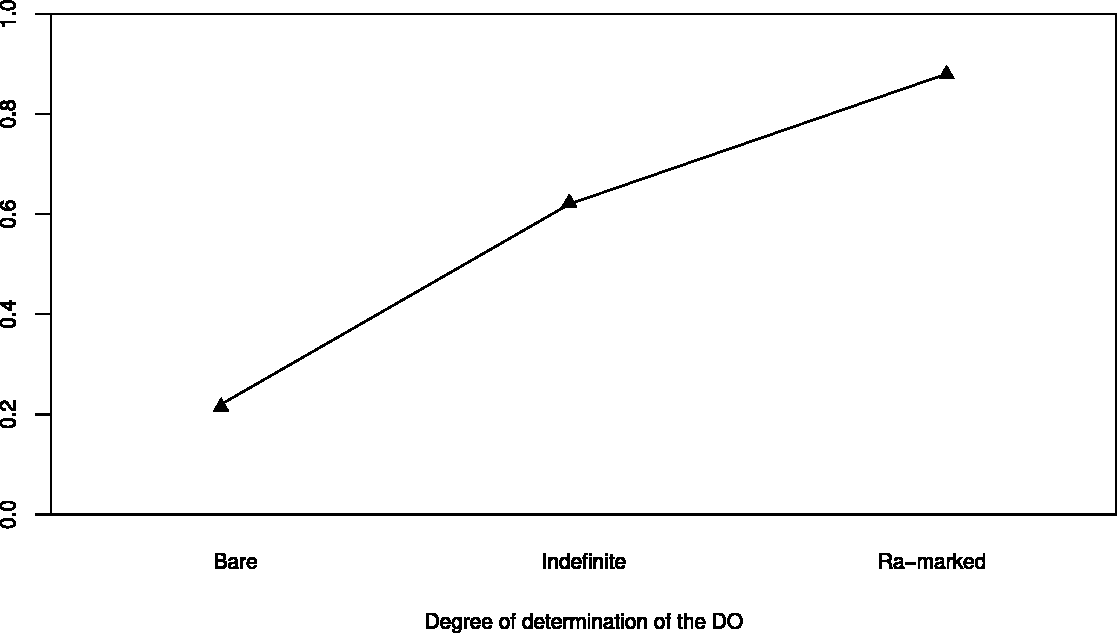
\includegraphics[width=\textwidth]{plots/Rplot01bis.pdf}
	\caption{Probability of the DO-IO-V order by the degree of determination of the DO}\label{Cline}
\end{figure}

Other important findings of these studies are:

\begin{itemize}\label{ListWOClaims}
	\item[d.]  Phrasal length (or heaviness) also plays a role in ordering preferences. The ``long-before-short'' preference is also observed in the preverbal domain in Persian, as in some other SOV languages such as Japanese \citep{hawkins94,yamashita2001}. Accordingly, ``heavy'' bare DOs, that is, bare-modified DOs, are less likely to appear adjacent to the verb than their ``light'' (single word) counterparts.
	\item[e.] The humanness of the IO favors the IO-DO-V order, which is in line with the general  ``animate-before-inanimate'' preference \citep{bresnan07,branigan1999conceptual,collins1995indirect,Hoberg81a,kempen2004corpus,Rosenbach2002}.
\end{itemize}



\section{Empirical study}

The review of the literature and the data discussed in previous sections show that in order to obtain an adequate account of the (in)separability of CP components we first need to get the empirical facts right. Most of the data provided in theoretical studies rely on ``informal'' anecdotal grammaticality judgements elicited without taking necessary methodological precautions and without any control for conflating factors. This undermines the empirical generalizations outlined in these studies, as shown by the abundance of counterexamples, some of which were given previously.  

Our aim is to achieve a better understanding of the issue at stake by adopting a quantitative approach that provides us with more reliable data and enables us to investigate and identify different factors that favor (non-)adjacency. The question under study is to what extent the nominal element of a CP, which is formally and syntactically comparable to the direct object (DO) of a lexical verb, is separable from the verb by a prepositional phrase, comparable to the indirect object (IO) of the same verb.


In this section, we present the results of two acceptability judgement experiments carried out as online questionnaires and filled out on a voluntary basis by native speakers of Persian living in Iran.

In both experiments, to obtain comparable data on word order variations in the preverbal domain, the questionnaire included (among other fillers) two additional series of experimental items, besides those for noun-verb CPs. One series focused on the relative order between the (bare) DO and the IO in ditransitive sentences and the other on the relative order of the subject and the (\textit{r\=a}-marked) DO in transitive sentences.\footnote{For each participant, the items were ordered in such a way that experimental items of each series were separated by other fillers: items of these different experiments were never presented in a successive order.}
Given that our first experiment serves as a pilot and that our two experiments are similar in many respects, we present and discuss these two additional series of items for the second experiment only. 

For noun-verb CPs, we compared sentences in which CP components appear in adjacent versus shifted orders, and manipulated the realization of the nominal element, comparing bare nouns with indefinite \textit{i}-marked NPs. 

We included a selection of CPs formed by concrete and predicative nouns\footnote{Note that our study did not include verbal nouns since, due to their limited nominal properties, they cannot develop into a DP/NP. However, their separability when they form a CP needs to be investigated in forthcoming studies.} that take a prepositional argument:\footnote{The above list includes all CPs used in our second experiment.}

\begin{description}\label{ListCP}
	\item CPs with concrete nouns: \textit{\=ab d\=adan} `to water' (water give), \textit{\=ah\=ar zadan} `to starch' (starch hit), \textit{qaz\=a d\=adan} `to feed' (food give), \textit{rang zadan} `to paint' (paint hit), \textit{rowqan zadan} `to oil' (oil hit), \textit{v\=aks zadan} `to polish' (polish hit),  \textit{v\=aksan zadan} `to vaccinate' (vaccination hit), \textit{namak zadan} `to salt' (salt hit).
	\item CPs with predicative nouns: \textit{foh\v{s} d\=adan} `to insult' (insult give), \textit{labxand zadan} `to smile' (smile hit), \textit{lagad zadan} `to kick' (kick hit), \textit{e\v{s}\=are kardan} `to point' (point do), \textit{ke\v{s}ide zadan} `to slap' (slap hit), \textit{kalak zadan} `to trick' (trick hit), \textit{\v{c}e\v{s}mqorre raftan} `to glare' (glare go), \textit{pok zadan} `to puff' (whiff hit).
\end{description}

All of these CPs display the syntactic pattern given in the canonical order in (\ref{CP-pattern}) and illustrated by (\ref{lbxndzd}).\footnote{We selected our CPs using the PersPred database \citep{SamFag2013}.}

\begin{exe}
	\ex\label{CP-pattern}
	N0($=$Subj) Prep~N1($=$IO) N2($=$DO)~Verb
	\ex\label{lbxndzd}
	\gll ali be maryam labxand zad\\
	Ali to Maryam smile hit.\gloss{pst.3sg}\\
	\glt	`Ali smiled at Maryam.'	
\end{exe}

Recall that while we agree with \citeauthor{Karimi-Doostan1997}'s judgements (see (\ref{kd-gush}c) above) on the impossibility for \textit{gu\v{s}} `ear' to project a DP/NP when part of the CP \textit{gu\v{s} d\=adan/kardan} `to listen', we do not endorse his generalization to the whole class of concrete (non-predicative) nouns. There are indeed examples of concrete nouns that can develop into a DP/NP in the context of a CP, such as those included in our selection. \textit{V\=aks} `polish', for instance, in the context of \textit{v\=aks zadan} `to polish' (lit. polish hit) (\ref{vakszdn}a), can head a DP/NP and be separated from the verb by a PP (\ref{vakszdn}b)?

\begin{exe}
	\ex\label{vakszdn}
	\begin{xlist}
		\ex[]{\gll  ali be kaf\v{s}-h\=a v\=aks zad\\
			ali to shoe-\gloss{pl} polish hit.\gloss{pst.3sg}\\
			\glt	`Ali polished the shoes.'}
		\ex[]{\gll ali behtarin v\=aks=r\=a be kaf\v{s}-h\=a zad\\
			Ali best polish=\gloss{ra} to shoe-\gloss{pl}  hit.\gloss{pst.3sg}\\
			\glt	`Ali polished the shoes with the best polish.'}
	\end{xlist}
\end{exe}

\begin{sloppypar}
  Moreover, the animacy/humanness of the referent of the prepositional
  argument was included in our experiments as a control variable, so
  that we could check whether the humanness of the IO favors the
  IO-DO-V order, as is suggested to be the case in ordinary
  ditransitive constructions in Persian (see
  page~\pageref{ListWOClaims}).
\end{sloppypar}
\begin{sloppypar}
  Our hypothesis is that the CPs of our sample do not differ from
  ordinary complement-verb combinations concerning word order
  variations. Therefore, based on the conclusions of
  \citet{FaghiriPhd} presented in Section~\ref{Sec:WO}, we predicted
  that:
\end{sloppypar}
\begin{enumerate}
	\item When the nominal element of the CP is realized as an indefinite NP, semantic relatedness favors the adjacent order, while the NP shift is licensed by the general tendency of indefinite DOs to precede the PP argument. 
	\item For bare nouns, both factors favor the adjacent order. 
	\item The phrasal length of the nominal element, that is, adding modification to the noun, favors separation.
	\item The humanness of the PP argument favors the adjacent order. 
\end{enumerate}

\subsection{Experiment 1 (pilot)}
\subsubsection{Method}
In our first (exploratory) experiment, we manipulated the nominal element on three levels: (a) bare noun, (b) indefinite \textit{i}-marked and (c) modified indefinite \textit{i}-marked. We prepared our material in such a way as to have a relatively natural and acceptable sentence  with all three forms of the nominal element in the condition of adjacent orders. To this end, we added a continuation to our target sentence, as in (\ref{fohs-exp}), specifically to improve the acceptability of sentences with indefinite \textit{i}-marked nominal elements.

We prepared 24 experimental items in six conditions according to Table~\ref{Tab:Exp1-Design}. In half of our stimuli, the PP argument was animate, as in (\ref{fohs-exp}) and (\ref{qaza-exp}), and in the other half, it was inanimate, as in (\ref{vaks-exp}). 
In 6 items, the nominal element was a concrete noun. The PP argument was animate only in one, \textit{qaz\=a d\=adan}, e.g.~(\ref{qaza-exp}). For the sake of space, only one version of each example is given here, the version corresponding to condition 6 in Table~\ref{Tab:Exp1-Design}, on the basis of which other versions can be constructed straightforwardly. 

\begin{table}
  \tabcolsep.4\tabcolsep %%% BC: this is intentional
	\begin{tabular}{lllcc}
      \lsptoprule 
		\multicolumn{3}{l}{} & \multicolumn{2}{c}{Order (adjacent vs. shifted)}\\\cmidrule(lr){4-5}
		\multicolumn{3}{l}{Type of the nominal element:} & [PP][NP] & [NP][PP]\\ 
		\midrule 
		bare &  \textit{foh\v{s}} & `insult' & 1 & 4\\ 
		\textit{i}-marked & \textit{foh\v{s}=i} & `an insult' & 2 & 5\\ 
		modified \textit{i}-marked & \textit{foh\v{s}=e rakik=i} & `a vulgar insult' & 3 & 6\\ 
    \lspbottomrule 
	\end{tabular}
	\caption{Experiment 1: Conditions\label{Tab:Exp1-Design}}
\end{table}

\begin{exe}
	\ex\label{fohs-exp}
	\gll sahar [foh\v{s}=e rakik=i] [be s\=ar\=a]   d\=ad va u=r\=a asab\=ani kard\\
	Sahar   insult=\gloss{ez} vulgar=\gloss{indf} to Sarah give.\gloss{pst.3sg} and him=\gloss{dom} angry do.\gloss{pst.3sg}\\
	\glt	`Sahar launched a vulgar insult to Sarah and made her angry.'
	
	\ex\label{qaza-exp}
	\gll ali   [qaz\=a=ye sabok=i] [be ba\v{c}\v{c}e-h\=a] d\=ad va anh\=a=r\=a be p\=ark bord\\
	Ali  food=\gloss{ez} light=\gloss{indf} to child-\gloss{pl}  give.\gloss{pst.3sg} and they=\gloss{ra} to park take.\gloss{pst.3sg}\\
	\glt	`Ali  gave the children some light food and took them to the park.'
	
	\ex\label{vaks-exp}
	\gll nima   [v\=aks=e si\=ah=i] [be kaf\v{s}-h\=a] zad va anh\=a=r\=a pu\v{s}id\\
	Nima  polish=\gloss{ez} black=\gloss{indf} to shoe-\gloss{pl}   hit.\gloss{pst.3sg} and they=\gloss{ra} wear.\gloss{pst.3sg}\\
	\glt	`Nima applied some black polish to the shoes and put them on.'
\end{exe}

The experiment was carried out as a web-based questionnaire (on \textit{Ibex Farm} \citep{ibex}) filled out by 37 native speakers. Participants were asked to rate each sentence on a Likert scale from 1 (absolutely unacceptable) to 7 (completely acceptable).

\subsubsection{Results}
\figref{boxplot} shows the distribution of the ratings by order (adjacent versus shifted) for the three realizations of the nominal element (bare, \textit{i}-marked and modified \textit{i}-marked). 

\begin{figure}[h]
    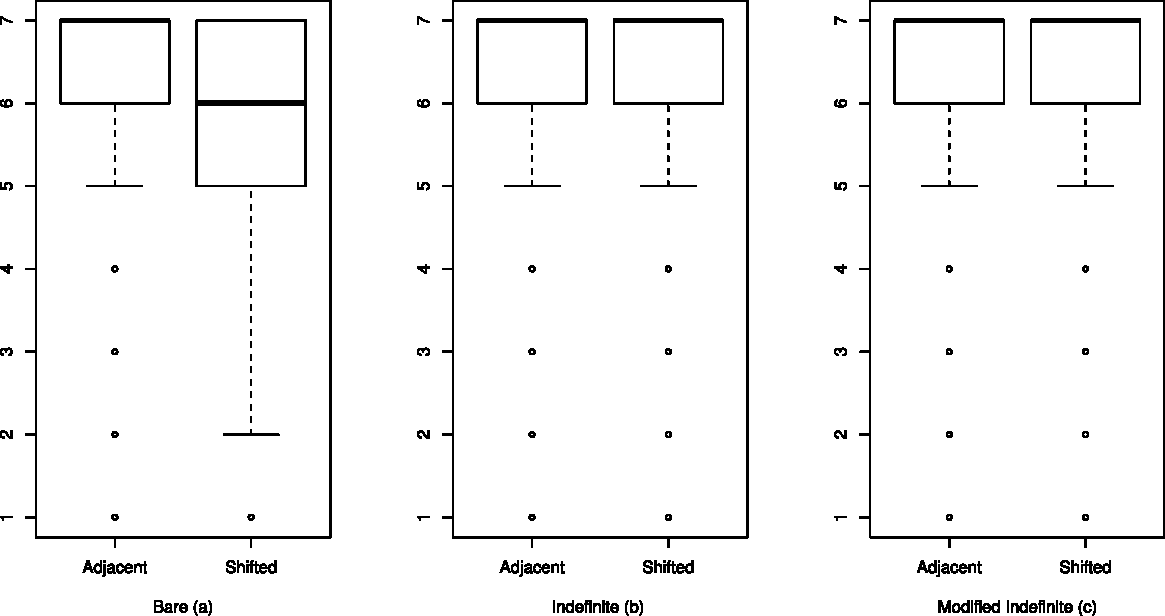
\includegraphics[width=1\linewidth]{plots/Rplot.pdf}
	\caption{Experiment 1: Distribution of ratings by order and type of nominal element}\label{boxplot}
\end{figure}

The statistical analysis of the results showed a significant difference in the ratings between adjacent ($\Mean=6.32, \SD=1.36$) and shifted orders ($\Mean=5.47, \SD=1.71$) only for bare nouns; $t(36)=5.05, p<0.001$.
%(LMM: $\hat{\beta}$ = -0.86, SE = 0.19, t = -4.57).%, p<.001).
The effect is, however, of medium size ($\text{Cohen's } d=0.53$) and shifted orders were overall rated as acceptable, as we see in Figure~\ref{boxplot}. 
For \textit{i}-marked (modified) NPs, both orders were similarly rated as highly acceptable, with mean rates above 6 %\footnote{6.23 (CI: $\pm$1.37) vs. 6.18 (CI: $\pm$1.38)} 
in all conditions, and we did not find any effect of phrasal length.

Concrete nouns of our sample display similar rating distributions. However, we will analyze this factor more thoroughly in the second experiment, in which the number of items is balanced for concrete and predicative nouns.

\begin{figure}
    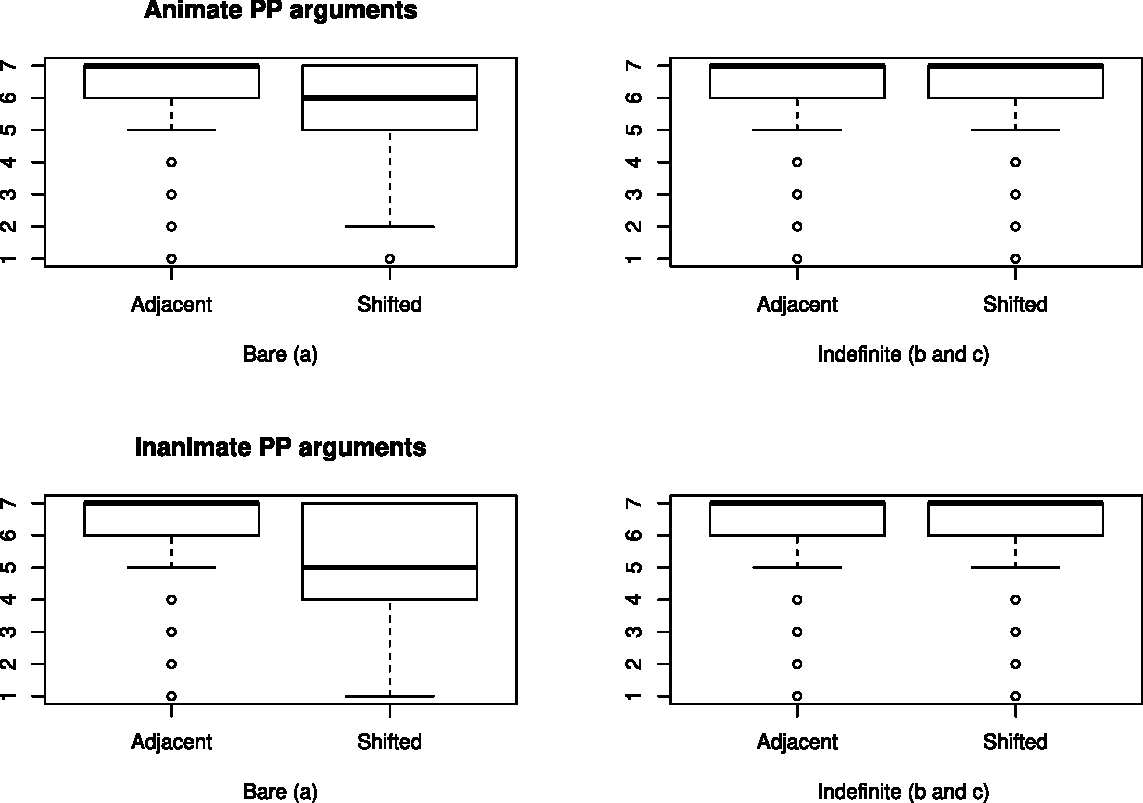
\includegraphics[width=1\linewidth]{plots/Rplot02-Exp1.pdf}
	\caption{Experiment 1: Distribution of ratings for animate versus inanimate PP arguments}\label{boxplot12}
\end{figure}

Interestingly, the humanness of the PP showed an impact on the ratings of sentences with bare nouns. As we can see in Figure~\ref{boxplot12}, animate PPs disfavored the shift more than inanimate PPs do. The statistical analysis, using a linear mixed-effects regression model with order and animacy as fixed effects and items and participants as random effects, showed a small but significant interaction between the two factors ($\text{Est.}= 0.26, \SE=0.07, t=3.44, p<0.01$). 


Overall, these results are in line with our predictions.  However,
ratings of ``non-canonical'' sentences were surprisingly high, that
is, rates below 4 were infrequent.  The fact that these sentences were
not rated as unacceptable may follow from \citet{FaghiriPhd} and
\citeauthor{FagSamHem2018}'s \citeyear{FagSamHem2018} observations
that the relative order between the NP and PP arguments is a matter of
soft constraints rather than a syntactic (phrase structure) rule.
Hence, while there is a clear bias in production towards a given
order, speakers do not consider the alternative order unacceptable (or
ungrammatical), and may, in some cases, even consider them equally
acceptable.  Nevertheless, to make sure that these results are not due
to an experimental confound, we replicated this experiment with a more
careful protocol.

\subsection{Experiment 2}
\subsubsection{Method}
In this experiment, we chose to keep lexical differences between items to a minimum level:
\begin{enumerate}
	\item Given that in Experiment 1 we did not find any differences between modified and single-word \textit{i}-marked nominal elements, we removed the modified \textit{i}-marked condition and manipulated the nominal element on two levels, bare versus indefinite \textit{i}-marked.
	
	\item Contrary to the previous experiment, we kept the sentence simple, that is, without any continuation. 
\end{enumerate}

We prepared 16 experimental items (15 from the previous experiment) in four conditions (see Table \ref{Tab:Exp2-Design}), as illustrated in examples (\ref{qaza-exp2}) -- (\ref{lgd-exp2}). 
In half of the stimuli, CPs were built with concrete nominal elements, and in the other half, with predicative nouns (see the list on page~\pageref{ListCP}). 
Two items with concrete nouns were built with animate PP arguments, e.g.~(\ref{qaza-exp2}), and six with inanimate PP arguments, e.g.~(\ref{ab-exp2}). 
Two items with predicative nouns were built with inanimate PP arguments, e.g.~(\ref{lgd-exp2}), and six with animate PP arguments, e.g.~(\ref{slm-exp2}).   For the sake of space, only one version of each example is given here, the version corresponding to condition 4 in Table~\ref{Tab:Exp1-Design}, on the basis of which other versions can be constructed straightforwardly.

\begin{table}
	\begin{tabular}{lllcc}
              \lsptoprule 
		\multicolumn{3}{l}{} & \multicolumn{2}{c}{Order (adjacent vs. shifted)}\\\cmidrule(lr){4-5} 
		\multicolumn{3}{l}{Type of the nominal element:} & [PP][NP] & [NP][PP]\\ 
		\midrule 
		bare & \textit{qaz\=a} & `food' & 1 & 3\\ 
		\textit{i}-marked &  \textit{qaz\=a=i} & `some food' & 2 & 4\\ 
		\lspbottomrule
	\end{tabular}
	\caption{Experiment 2: Conditions}\label{Tab:Exp2-Design}
\end{table}

\begin{exe}
	\ex\label{qaza-exp2}
	\gll ali [qaz\=a=i] [be ba\v{c}\v{c}e-h\=a]    d\=ad\\
	Ali food=\gloss{indf} to child-\gloss{pl}  give.\gloss{pst.3sg}\\
	\glt	`Ali gave some food to the children.'
	
	\ex\label{ab-exp2}
	\gll maryam   [\=ab=i] [be b\=aq\v{c}e] d\=ad\\
	Maryam  water=\gloss{indf} to garden give.\gloss{pst.3sg}\\
	\glt	`Maryam (lit.) gave some water to the garden.'

	\ex\label{slm-exp2}
	\gll s\=ar\=a  [labxand=i] [be mehm\=an-h\=a]  zad\\
	Sarah smile=\gloss{indf} to guest-\gloss{pl}  hit.\gloss{pst.3sg}\\
	\glt	`Sarah (lit.) gave a smile to the guests.'

	\ex\label{lgd-exp2}
	\gll omid [lagad=i] [be dar] zad\\
	Omid  kick=\gloss{indf} to door hit.\gloss{pst.3sg}\\
	\glt	`Omid  gave a kick to the door.'
\end{exe}

Beside these target sentences, our stimuli included four series of control items as fillers (two series of unacceptable control sentences and two series of experimental items on word order variation):

\begin{enumerate}\label{ListFiller}
	\item 8 sentences with clear grammaticality violations, such as (\ref{cont2-exp2}).
	
	\begin{exe}
		\ex[*] {\gll ... di\v{s}ab b\=ar\=an=r\=a  zi\=ad \=amad\\
			{} last-night rain=\gloss{ra} very come.\gloss{pst.3sg}\\
			\glt	Intended:`... it rained a lot last night.'\label{cont2-exp2}}   
	\end{exe}
	
	\item  2 sentences similar to the example (\ref{kd-gush-ind}) above by \citeauthor{Karimi-Doostan:2011}: 
	
	\begin{exe}
		\ex\label{cont1-exp2}
		\gll ... amir  [gu\v{s}=e b\=a-deqqat=i]  [be mo'alem] d\=ad\\
		{} Amir ear=\gloss{ez} careful=\gloss{indf} to teacher give.\gloss{pst.3sg}\\
		\glt	Intended:`... Amir listened carefully to the teacher.'	

		\ex\label{cont12-exp2} 
		\gll ... neda  [\v{c}e\v{s}m=e moztareb=i]  [be \v{c}amed\=an] and\=axt\\
		{}  Neda eye=\gloss{ez} worried=\gloss{indf} to suitcase launch.\gloss{pst.3sg}\\
		\glt	Intended:`... Neda looked worriedly at the suitcase.'		
	\end{exe}
	
	\item 8 experimental items, similar to (\ref{cont3-exp2}), focusing on the relative order between the subject and the \textit{r\=a}-marked DO in prototypical transitive sentences.\footnote{These items are taken from  \citeauthor{FaghiriPhd}'s (\citeyear{FaghiriPhd}) sentence completion experiment on transitive sentences (see Experiment T1 (pp.~197--204)).}
	
	\begin{exe}
		\ex\label{cont3-exp2}
		\begin{xlist}
			\ex[]{\gll ... omid maryam=r\=a n\=ar\=ahat kard\\
				{...} Omid Maryam=\gloss{ra} hurt do.\gloss{pst.3sg}\\
				\glt	`... Omid hurt Maryam.'
			}		
			\ex[]{... maryam=r\=a omid n\=ar\=ahat kard}			
		\end{xlist}
	\end{exe}
	
	\item 16 experimental items, similar to (\ref{cont4-exp2}) and (\ref{cont42-exp2}), focusing on the relative order between the IO and a bare DO\footnote{In this experiment, we also manipulated the phrasal length of the DO, comparing bare and bare modified nouns. Here we only discuss the data for bare DOs.} with control for the humanness of the IO.\footnote{These items are taken from  \citeauthor{FaghiriPhd}'s (\citeyear{FaghiriPhd}) sentence completion experiments on ditransitive sentences (see Experiment D2 (pp.~178--193) and Experiment D4 (pp.~188--193)).}
	
	\begin{exe}
		\ex\label{cont4-exp2}
		\begin{xlist}
			\ex[]{\gll ... sar=e miz gol be-goz\=ar-and\\
				{} on=\gloss{ez} table flower \gloss{sbj}-put.\gloss{prs-3pl}\\
				\glt	`... (they) put flowers on the table.'
			}		
			\ex[]{ ... gol sar=e miz be-goz\=ar-and}
		\end{xlist}

		\ex\label{cont42-exp2}
		\begin{xlist}
			\ex[]{\gll ... bar\=a=ye soxanr\=an \v{c}\=ay bi-\=avar-and\\
				{} for=\gloss{ez} speaker tea \gloss{sbj}-bring.\gloss{prs-3pl}\\
				\glt	`... (they) bring tea for the speaker.'
			}		
			\ex[]{ ... \v{c}\=ay bar\=a=ye soxanr\=an  bi-\=avar-and}
		\end{xlist}
	\end{exe}
	
\end{enumerate}

The remaining 30 fillers covered a range from highly acceptable to less acceptable sentences.


The experiment was again carried out as a web-based questionnaire. However, unlike the previous experiment, we opted for an 11-point scale from 0 (absolutely unacceptable) to 10 (completely acceptable), which we consider to be more natural for our participants than a 7-point scale. Also, the rating task was followed by comprehension questions in 40 filler items. 

116 monolingual speakers of Persian living in Iran filled out the questionnaire. We discarded answers from three participants who had more than 10\% of wrong answers to comprehension questions and/or rated clearly ungrammatical sentences as acceptable. Our final dataset hence contained a total number of 1808 observations. 

\subsubsection{Results}
The distribution of ratings by experimental condition in our target items is given in \figref{boxplot1}. Figure~\ref{boxplot2} shows the distribution of ratings for our clearly unacceptable control items (1 and 2 on page \pageref{ListFiller}).


\begin{figure}
	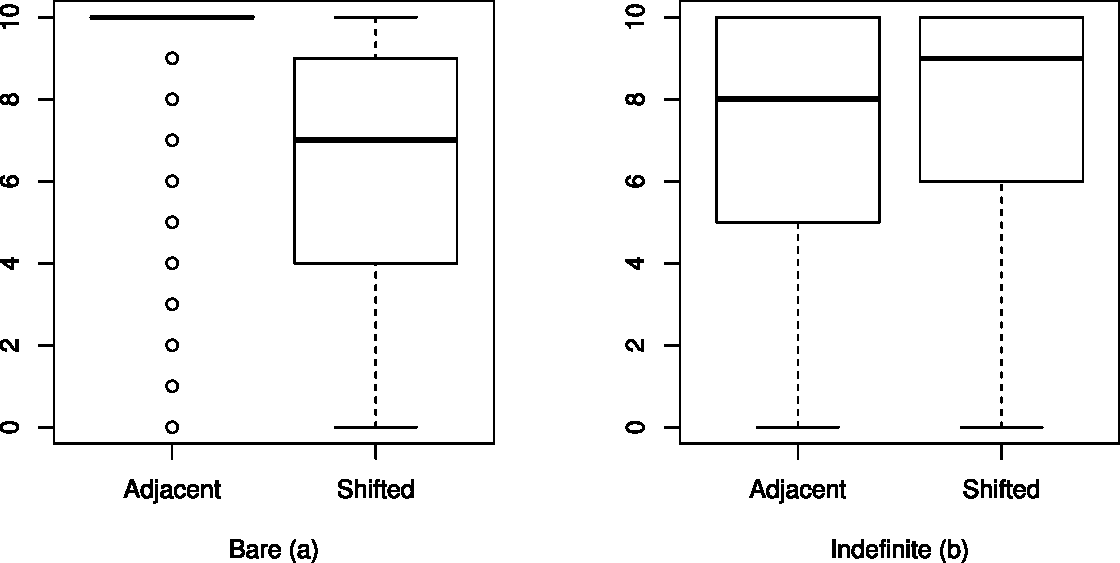
\includegraphics[width=1\linewidth]{plots/Rplot04.pdf}
	\caption{Experiment 2: Distribution of ratings by experimental condition}\label{boxplot1}
\end{figure}

\begin{figure}
    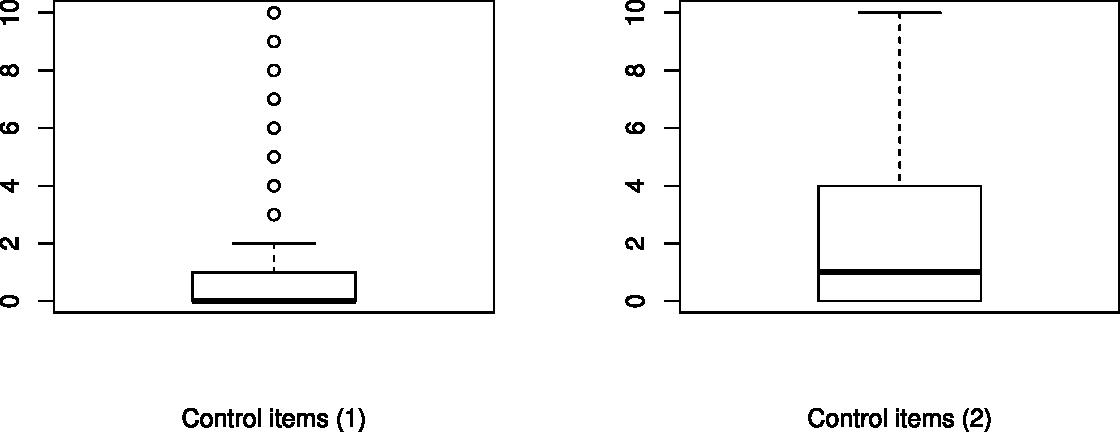
\includegraphics[width=1\linewidth]{plots/Rplot05.pdf}
	\caption{Experiment 2: Distribution of ratings for clearly unacceptable control items}\label{boxplot2}
\end{figure}

We can see that the distribution of ratings in our new data is not substantially different from Experiment 1.
Here again, the distribution of ratings is (almost)\footnote{Interestingly, the mean is slightly but significantly better for shifted orders: 7.59 ($\SD=2.85$) vs. 7.14 ($\SD=3.05$); $t(112)=3.24$, $p<0.01$.} identical for the two orders in the case of indefinite \textit{i}-marked NPs and the analysis of the results shows a significant decrease for shifted orders ($\Mean=6.49, \SD=3.07$) compared to adjacent orders ($\Mean=9.27, \SD=1.87$) only for bare nouns; $t(112)=13.43, p<0.001$. The effect size is large ($\text{Cohen's } d=0.96$) and much more important than what we had previously. Nevertheless, sentences in the shifted order were still not rated as unacceptable: the median  is 7. Compare the distribution of ratings in target items with our clearly unacceptable controls where both mean and median are very low: respectively 2.4 and 1 for the first set of control items, and 1.2 and 0 for the second ones.
It is also instructive to take a closer look at the frequency distribution of ratings for adjacent versus shifted orders, compared to our unacceptable controls (see \figref{barplot1}).  In sharp contrast to the latter, high scores remained the most frequent ratings for shifted orders and the mode is still 10.
Indeed, we do not have a bi-modal distribution, with some speakers rating these sentences as totally unacceptable and others as perfectly acceptable. Speakers mostly tended to rate these sentences as equally acceptable or slightly less acceptable than canonical sentences.

\begin{figure}[h]
          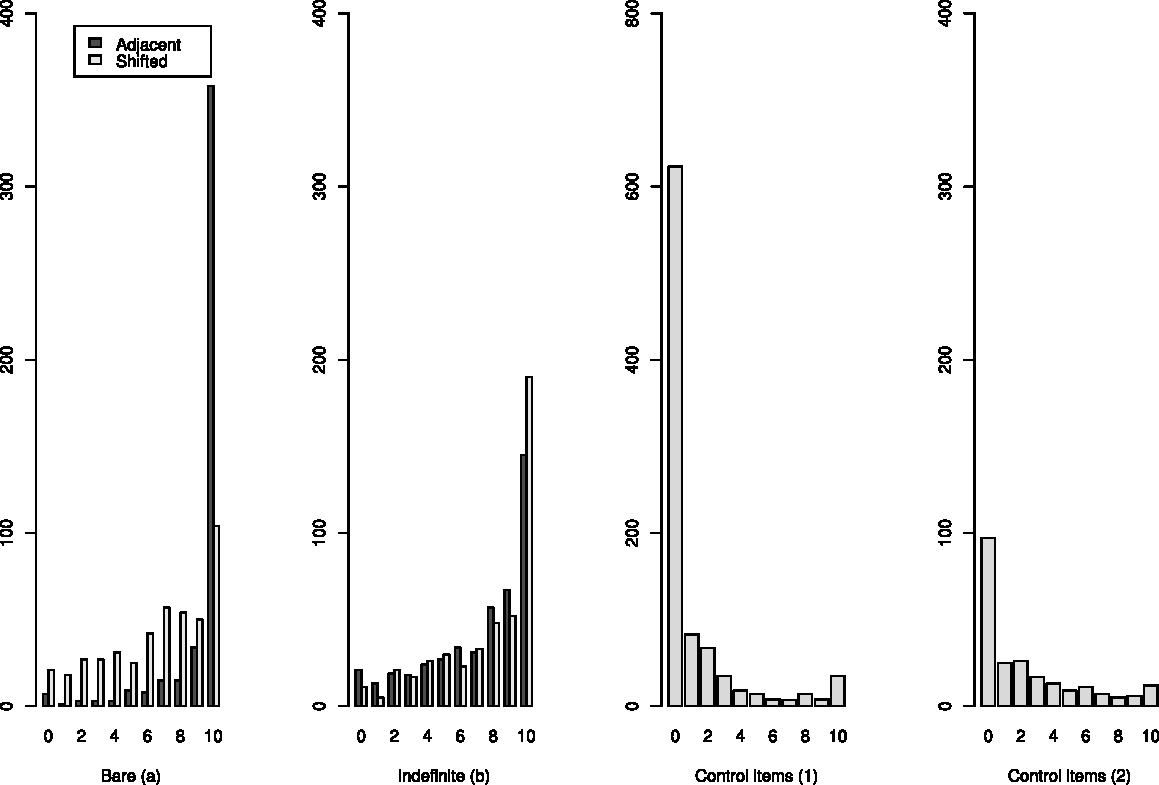
\includegraphics[width=\textwidth]{plots/Rplot06.pdf}
	\caption{Experiment 2: Frequency distribution of ratings for target items versus unacceptable control items}\label{barplot1}
\end{figure}

\begin{figure}
    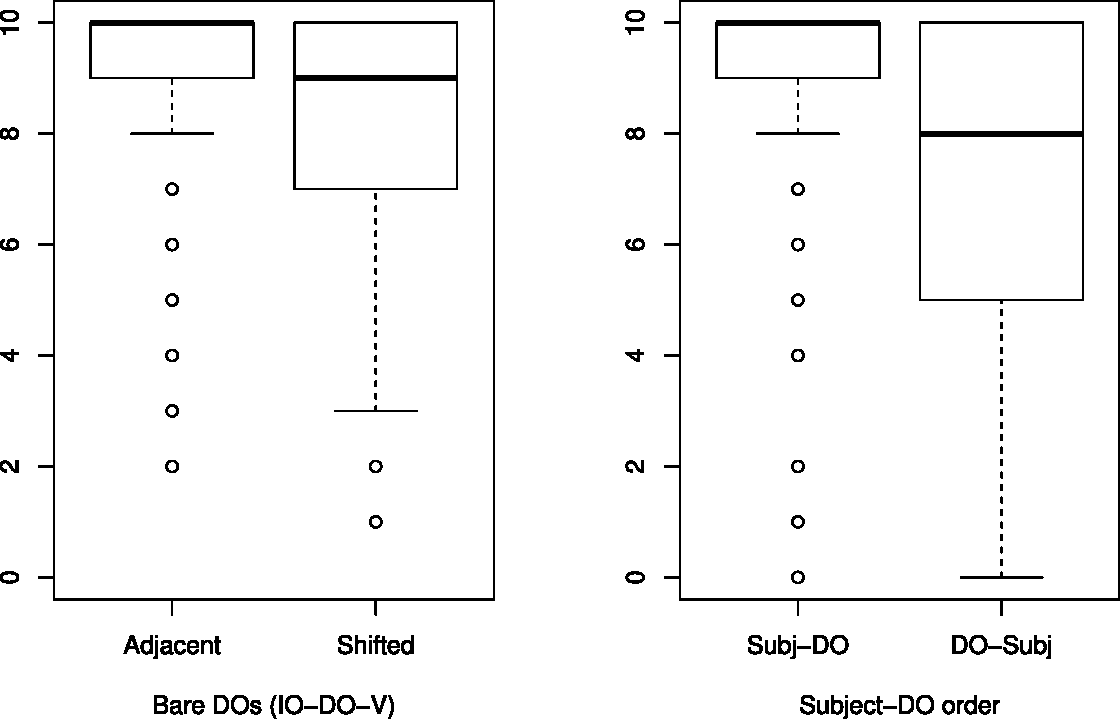
\includegraphics[width=1\linewidth]{plots/Rplot07.pdf}
	\caption{Experiment 2: Distribution of ratings for word order variation control items}\label{boxplot4}
\end{figure}


At this point, let us compare these data with our two other series of experimental items on word order variations, that is, 1) the relative order between the (bare) DO and the IO, and 2) the relative order between the subject and the DO in prototypical transitive sentences (see the box and whisker diagrams in Figure~\ref{boxplot4}). In both cases, we find a significant decrease in the mean rating for ``non-canonical'' orders as well. However, the effect sizes are smaller and ``non-canonical'' orders were rated relatively better than what we observe for CPs (with bare nominal elements).  
In the case of the relative order in transitive sentences, the effect is of medium size ($\text{Cohen's } d=0.73$), the difference between the mean rating for canonical (Subj-DO) and non-canonical (DO-Subj) orders is less than 2 points (9.19 vs. 7.34; $t(112)= 10.46, p<0.001$), and the median rating for non-canonical orders is 8. 
Interestingly, for bare DOs, the effect size is small -- half the size we had for bare nouns forming a CP ($\text{Cohen's } d=0.48$). The difference between the mean rating  for adjacent and shifted orders is almost 1 point (9.33 vs. 8.42; $t(112)= 7.48, p<0.001$) and the median rating for shifted orders is 9. 


Finally, let us consider the effect of our two control factors: 1) the type of the nominal element and 2) the humanness of the PP argument. Figures~\ref{boxplot3} and~\ref{boxplot5} provide the same box-and-whisker diagrams of the distribution of ratings, respectively, for concrete versus predicative nominal elements, and for animate versus inanimate PP arguments. 


\begin{figure}
	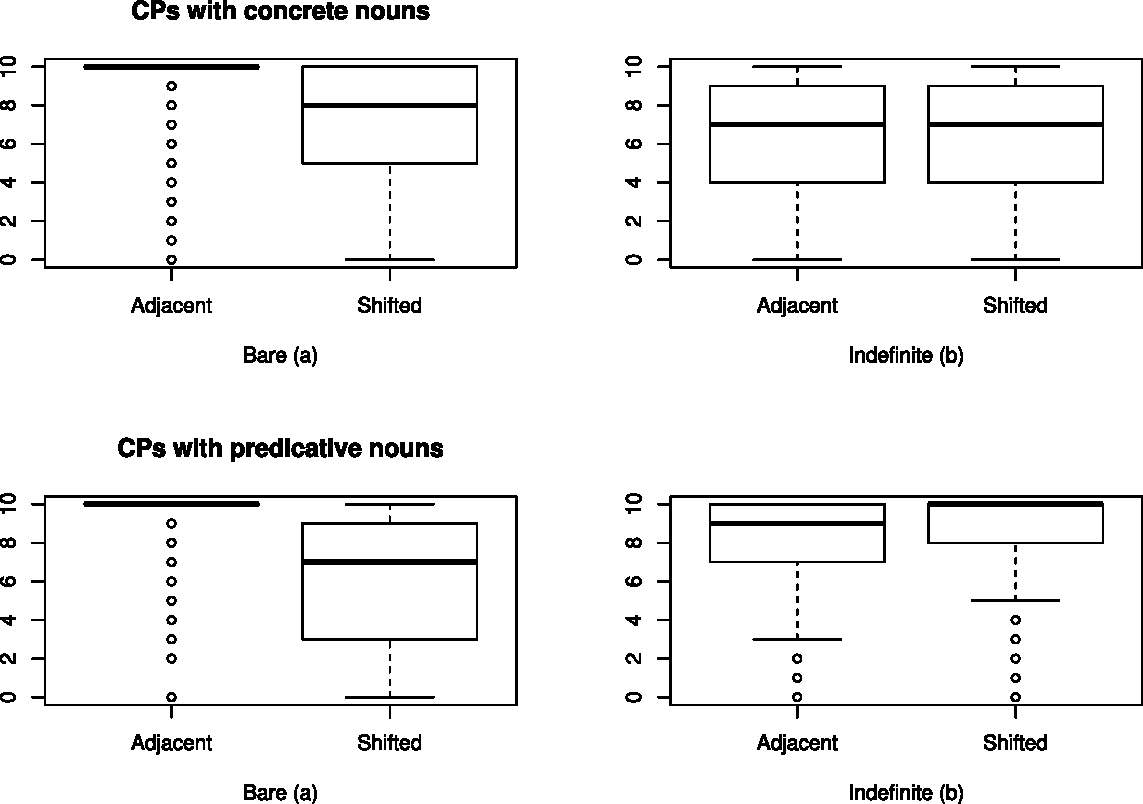
\includegraphics[width=1\linewidth]{plots/Rplot03.pdf}
	\caption{Experiment 2: Distribution of ratings by (semantic) type of the nominal element}\label{boxplot3}
\end{figure}

\begin{figure}
	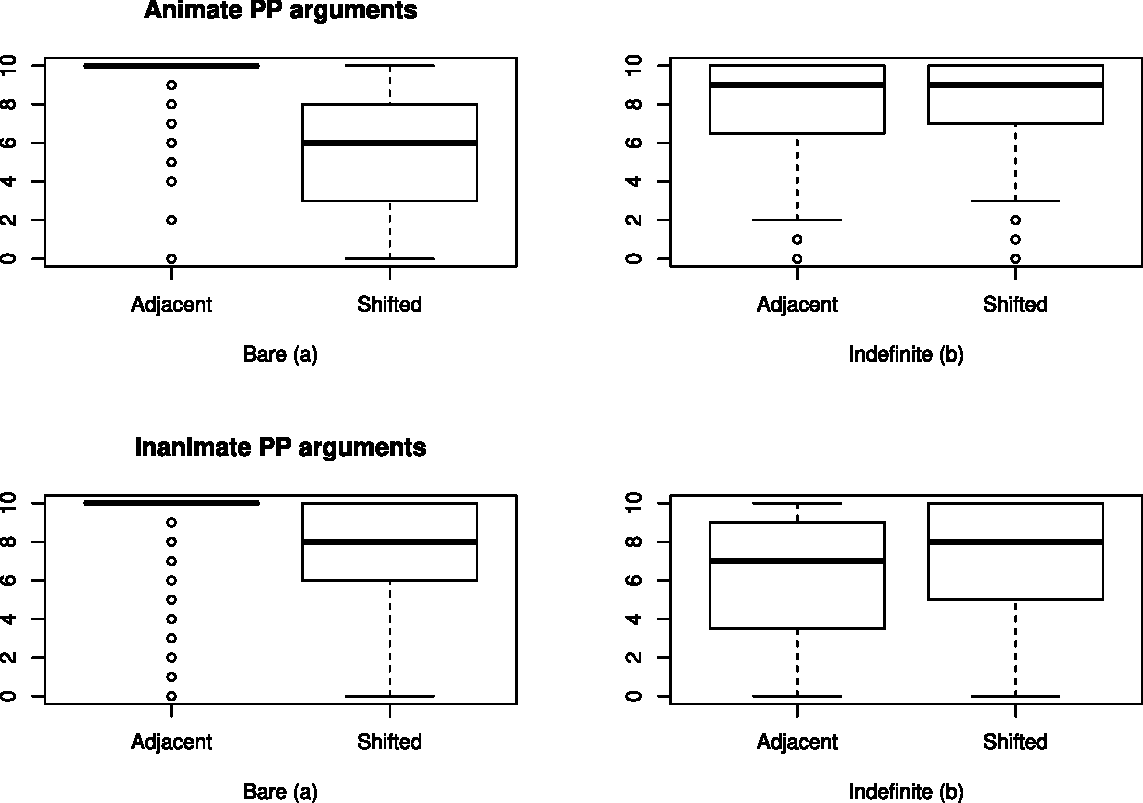
\includegraphics[width=1\linewidth]{plots/Rplot02-Exp2.pdf}
	\caption{Experiment 2: Distribution of ratings by animacy (of the PP argument)}\label{boxplot5}
\end{figure}



Recall, however, that these two factors are correlated in our design. Hence, we need to look at the linear mixed-effects model (LMM) analyses of the data \citep{baayen2008mixed} in order to be able to capture the effect of these two factors on acceptability judgements independently and in interaction with order. To this end, ratings were entered into a mixed-effect linear regression model using the lme4 package \citep{bates2015lme4} of the R statistics software (R Core Team 2016). We ran two separate models, one including only bare nouns and the other indefinite \textit{i}-marked NPs. In each model, the experimental factors are included as fixed effects, with sum-coded contrasts.\footnote{Order: $\text{Adjacent}=1$, $\text{Shifted}=-1$; Animacy: $\text{Animate}=1$, $\text{Inanimate}=-1$: Noun-Type: $\text{Predicative}=1$, $\text{Concrete}=-1$.} We fitted the full variance-covariance structure of random effects for both items and participants, justified by the design.  
Table~\ref{Tab:Res-BN} presents the summaries of both models for fixed effects. The results are as following:

\begin{enumerate}
	\item The estimated mean (baseline) rating across all factors is above 7 in both cases (7.81 and 7.29, for bare nouns and indefinite NPs respectively).
	
	\item As expected, there is a significant and relatively important main effect of order for bare nouns: the difference in the (estimated) mean rates between adjacent and shifted orders is about 3 points. 
	However, in the case of indefinite NPs, the effect of order, while significant, is very small and, interestingly, goes in the opposite direction. The difference in the (estimated) mean scores between shifted and adjacent orders is only about 0.5 point. 
	
	\item There is a significant but rather small interaction between order and animacy for both bare nouns and indefinite NPs: with shifted orders, inanimate PPs yield slightly better scores than animate PPs.  
	
	\item There is no interaction between Order and Noun-Type, neither for bare nouns nor for \textit{i}-marked NPs. For the latter, however, Noun-Type has a significant and relatively important main effect on the ratings: predicative nominal elements are rated better than concrete ones regardless of order. The difference in the (estimated) mean  scores between the two noun types is about 2 points.
\end{enumerate}

\begin{table}
  \subfigure[Bare nouns]{%
	\begin{tabular}{l S[table-format=+1.2] S[table-format=1.2] S[table-format=2.2] S[table-format=+1.2] S[table-format=<1.3] l}
          \lsptoprule
		& {Est.} & {SE} & {df} & {$t$} & {$p$} & \\
		\midrule
		Intercept  					      & 7.81   &  0.24 &  26.03 & 23.74  & <0.001 & ***\\ 
		\textsc{order [adjacent=1]}       & 1.47   & 0.11  &  40.12 & 12.64  & <0.001 & ***\\ 
		\textsc{animacy [animate=1]}      & -0.21  & 0.24  & 14.25  &  -0.91 & 0.38 & \\
		\textsc{nountype [predicative=1]} & -0.10  & 0.23  & 13.48  & -0.45  & 0.66  & \\
		\textsc{order:animacy} 		      &  0.40  & 0.10  & 14.73  & 3.85   & <0.01 & **\\
		\textsc{order:nountype} 		  &  0.02  & 0.10  & 11.54  & 0.17   & 0.87 & \\
          \lspbottomrule
        \end{tabular}
      }
      \subfigure[Indefinite \textit{i}-marked NPs]{%
      \begin{tabular}{l S[table-format=+1.2] S[table-format=1.2] S[table-format=2.2] S[table-format=+1.2] S[table-format=<1.3] l}
        \lsptoprule
		& {Est.} & {SE} & {df} & {$t$} & {$p$} &\\
		\midrule
		Intercept  					& 7.29    &  0.26 &  46.16 & 28.16& <0.001 & ***\\ 
		\textsc{order [adjacent=1]}  &    -0.23 & 0.09 &  11.65 & -2.61   & <0.05 & *\\ 
		\textsc{animacy [animate=1]}    &   0.04  & 0.22  & 14.79 & 0.21 & 0.84 & \\
		\textsc{nountype [predicative=1]} &  1.07 & 0.22 & 16.97 & 4.78 & <0.001 & ***\\
		\textsc{order:animacy} 		&  0.35 & 0.13 & 18.13 & 2.80  & <0.05 & *\\
		\textsc{order:nountype} 		&  -0.07 & 0.11  & -0.59 & 0.17 & 0.57 & \\
          \lspbottomrule
      \end{tabular}}
	\caption{Experiment 2: Results of LMM analyses}\label{Tab:Res-BN}
\end{table}


\subsection{Main findings}

The main findings of our experimental study are:

\begin{enumerate}
	\item Sentences in which bare nouns forming a CP appear separated from the verb by the PP argument are not considered to be ungrammatical by native speakers, but only less acceptable than sentences in which they appear adjacent to each other. 
	However, in comparison, ordinary ditransitive sentences in which the bare noun is separated from the verb by the PP argument are rated better.
	
	\item When the nominal element of a CP is realized as an indefinite \textit{i}-marked NP, sentences in which the nominal element is separated from the verb by the PP argument are considered slightly more acceptable.
	
	\item The predicative nature of the noun forming a CP has no effect on ordering preferences. In other words, speakers accept sentences in which concrete nouns are separated from the verb in the same manner as they accept those with predicative nouns. 
	Meanwhile, as expected, the ability of the nominal element of a CP to develop a DP projection is affected by its predicative nature: when the nominal element was \textit{i}-marked, CPs of our sample formed by predicative nouns were rated better than those formed by concrete nouns.
	
	\item The humanness of the intervening PP argument disfavors the separability of CP components: sentences in which the nominal element precedes the PP were rated slightly better when the PP argument was inanimate than when the PP argument was human.
\end{enumerate}

In a nutshell, the findings of our study contradict all previous claims on the inseparability of CP components \citep[e.g.][]{Goldberg1996,Karimi-Doostan1997,Karimi-Doostan:2011} and suggest not only that ``real'' syntactic material can interrupt a noun-verb CP but also that ordering preferences in CPs are comparable to those observed in ordinary complement-verb combinations, semantic relatedness and collocationality put aside. 

Before closing this section, it is important to discuss a previous quantitative evaluation of Karimi-Doostan's claim on the (in)separability of CP components, which arrives at a different conclusion, partially at odds with the conclusions of our study.

In a recent paper on language processing, \citet{SafaviEtal2016} use separable Persian CPs to test the predictions of different accounts of locality effects and follow \citeauthor{Karimi-Doostan:2011}'s classification to select separable CPs. In order to make sure that the CPs included in their experimental material are separable for native speakers they carried out a preliminary norming acceptability rating experiment to test the relative acceptability of ``separable'' versus ``inseparable'' CPs (\citeyear[4]{SafaviEtal2016}). 
They had 50 native speakers rate three sets of 36 sentences with CPs from each class, following a between-items design with three conditions: (a) verbal nouns, (b) predicative nouns and (c) non-predicative nouns, and report the following mean rates on a 7-point Likert scale, respectively: 3.23 ($\text{Q1}=1, \text{Q3}=5$), 6.08 ($\text{Q1}=6, \text{Q3}=7$), and 3.12 ($\text{Q1}=1, \text{Q3}=5$), that suggest a clear-cut distinction between ``separable'' and ``inseparable'' CPs in support of \citeauthor{Karimi-Doostan1997}'s classification.

Nevertheless, a closer look into their stimuli, provided on-line as supplementary material,\footnote{Accessible via the following link: http://journal.frontiersin.org/article/10.3389/fpsyg2016.00403} shows that they did not perform a systematic (minimally paired) comparison across the three conditions. 
An example of items in each condition is given in~(\ref{safavi-exp}).\footnote{Glossing and translations are ours.}

\begin{exe}
	\ex\label{safavi-exp}
	\begin{xlist}
		\ex[]{\gll hamk\=ar=am n\=ame=i \emph{ers\=al} [be man] kard\\
			colleague=\gloss{cl.3sg} letter=\gloss{indf}  sending to me do.\gloss{past.3sg}\\
			\glt	`My colleague sent me a letter.'
		}
		
		\ex[]{\gll maryam \emph{arezu=i} [bar\=a=ye man] kard\\
			Maryam  wish=\gloss{indf} for I do.\gloss{past.3sg}\\
			\glt	`Maryam made a wish for me.'
		}
		\ex[]{\gll golnaz \emph{otu} [be leb\=as=a\v{s}] zad\\
			Golnaz  iron to dress=\gloss{cl.3sg} hit.\gloss{past.3sg}\\
			\glt	`Golnaz ironed her dress.'
		}
	\end{xlist}
\end{exe}

We notice that while the indefinite \textit{i}-marked form is used in sentences with predicative nouns, as in (\ref{safavi-exp}b), the bare form is used for the other classes, as in (\ref{safavi-exp}a) and (\ref{safavi-exp}c). This is not surprising given that, as we have seen in Section~\ref{Sec:Severing},  the issue of (in)separability is entangled with the realization of the NP (or the ability of the nouns to develop a DP/NP projection) in \citeauthor{Karimi-Doostan1997}'s view. However, this design makes the comparison between the three conditions meaningless. 

Putting aside verbal nouns that cannot develop a DP/NP projection, we have seen that in a number of CPs involving a non-predicative noun, the nominal element can develop a DP/NP projection and be separated from the verb. However, \citeauthor[]{SafaviEtal2016} did not control for this property in their design and in a number of their items involving a non-predicative noun, such as \textit{otu zadan} `to iron' (iron hit) in (\ref{safavi-exp}c), the nominal element can appear in the \textit{i}-marked form, as illustrated in (\ref{safavi-exp-contr}), while they also include CPs such as \textit{gu\v{s} d\=adan} `to listen' (ear give).

\begin{exe}
	\ex\label{safavi-exp-contr}
	\gll golnaz \emph{otu=i} be leb\=as=a\v{s} zad\\
	Golnaz  iron=\gloss{indf} to dress=\gloss{cl.3sg} hit.\gloss{past.3sg}\\ 
	\glt	`Golnaz ironed her dress.'
\end{exe}

Note that the stimuli include only one version of each item: a sentence in which the noun is separated from the verb by a prepositional phrase and there is no control on the function and semantics of the intervening PP. 
As a consequence, while their data serve the initial purpose of their norming pretest, they do not provide evidence for the inseparability of CPs with non-predicative nouns (in opposition to CPs with predicative nouns).

\section{Conclusions}

\begin{sloppypar}
  The experimental data presented in the previous section 1) provide
  additional support, along with the attested counterexamples given in
  Section~\ref{Sec:Severing} and in \citet{Samvelian2012}, that the
  nominal element of a CP, whatever its form and its type, can be
  separated from the verb by syntactic material, and 2) suggest that
  the issue of separability in CPs cannot be studied separately from
  word order preferences involving the verb and its complements in
  ordinary transitive and ditransitive constructions.
\end{sloppypar}

Our study constitutes a first step in the study of the issue of separability with quantitative and experimental methods. Further studies are needed in order to investigate several points that we did not address in this paper: 

\begin{description}
\item[Production data:] Our study suggests that speakers have an important tolerance for sentences in which the bare nominal element is separated from the verb by the PP argument of the CP, since, as explained in the previous section, acceptability rates stay high, that is, clearly above the baseline. In order to have a more accurate picture, the acceptability judgement data must be completed by production data, including corpus studies. 

\item[Separation by constituents other than PP arguments:]
  \begin{sloppypar}
    Our experiments were designed with sentences in which the
    intervening element was the PP argument of the CP since our
    purpose was to assess Karimi-Doostan's claim on separability. The
    possibility for other constituents, such as adverbials, to
    intervene between the nominal element and the verb must be
    investigated in forthcoming studies. However, we should emphasize
    that such an investigation must include an examination of the same
    possibilities in ordinary object-verb combinations, particularly
    in the case of bare objects. Recall from Section~\ref{Sec:WO}
    that, as mentioned in several studies, a bare object of lexical
    verbs also displays a limited degree of autonomy with respect to
    the verb and tends to occur adjacent to the latter.
  \end{sloppypar}
\item[Separability and DP projection:]
  \begin{sloppypar}
    All examples in our data were designed with nouns that can project
    NP/DPs, be they predicative or concrete, since the purpose was not
    only to check the possibility for bare nouns to be separated from
    the verb but also to study the role of the degree of determination
    in ordering preferences. However, not all concrete nouns can
    project a DP/NP when forming a CP. Recall the example of
    \textit{gu\v{s}} `ear' in \textit{gu\v{s} d\=adan/kardan} `to
    listen' (ear give/do) given by Karimi-Doostan. Although we did not
    include these cases in our experiments, it seems safe to consider
    that their behavior (as bare nouns) should not be different from
    those that can project a DP/NP in the context of a given CP. Note
    that examples of separation for \textit{gu\v{s} d\=adan/kardan}
    abound in the literature. Here are a few of them:
  \end{sloppypar}

\end{description}

\begin{exe}
	\ex
	\gll abbas n\=ar\=ahat va pa\v{z}morde bud. gu\v{s} be m\=adar=a\v{s} d\=ad...\\
	Abbas sad and unhappy was ear to mother=\gloss{cl.3sg} give.\gloss{pst.3sg}\\
	\glt`Abbas was sad and unhappy. He listened to his mother...' 	\hfill (Ali A\v{s}raf Darvi\v{s}ian, \textit{Jang be rev\=ayat-e ba\v{c}\v{c}eh\=a}, p.~30) 
	\ex
	\gll gu\v{s} be harf=e man bo-kon ... va baqi=r\=a vel-kon...\\
	ear to speech=\gloss{ez} \textsc{1.sg} \gloss{imp}-do\gloss{.2sg} {} and rest=\gloss{ra} leave.\gloss{imp.2sg}\\
	\glt`Listen to me (...) and let go of the rest...' 	\hfill (\v{S}irin Sami'i, \textit{Bibi va touti}, p.~44) 
\end{exe}

Apart from non-projecting concrete nouns, we also excluded verbal
nouns, e.g. \textit{ers\=al} `sending', from our study. Recall that the
latter display limited nominal properties and can never be determined,
whether in the context of a CP or not. It seems that verbal nouns resist separation more than predicative and concrete nouns. Although this fact
needs to be checked by further empirical studies, it would not be
surprising a priori. Indeed, the problematic status of these ``nouns''
can account for the fact that they are not perceived as direct objects
and consequently are not subject to the same ordering variations.

To conclude, Persian CPs, like other types of multiword expressions in
various languages, illustrate a case of deviation from the one-to-one
mapping of form and meaning. Even though they realize a
single semantic unit, their components nevertheless enjoy the mobility
granted to members of ``ordinary'' verb-complement syntactic
constructions and are subject to the same constraints with respect to the
linear order. The semantic bond nevertheless plays a role in granting
CPs hallmarks of ``wordhood'', favoring their adjacency, among other
things.

\section*{Abbreviations}
Glosses follow the Leipzig Glossing Rules. The following non-standard abbreviations are used for clarity:  

\begin{tabbing}
SINF\quad\= short infinitive\kill
EZ   \> Ezafe\\
RA   \> differential object marker\\
SINF \> short infinitive
\end{tabbing}

\section*{Acknowledgements}
\begin{sloppypar}
  We are grateful for feedback at the following conferences and
  workshops: Linguistic Evidence (Tübingen, February 2018), ConCALL
  (Bloomington, March 2018) and EW-HPSG (Frankfurt, June 2018). We
  would also like to thank Berthold Crysmann, Manfred Sailer and the
  anonymous reviewers for their comments and suggestions.  This work
  is partially supported by a public grant overseen by the French
  National Research Agency (ANR) as part of the program
  ``Investissements d’Avenir'' (reference: ANR-10-LABX-0083). It
  contributes to the IdEx Université de Paris (ANR-18-IDEX-0001).
  This work was completed while the first author held a postdoctoral
  position at Universität zu Köln.
\end{sloppypar}
{\sloppy\printbibliography[heading=subbibliography,notkeyword=this]}

\end{document}
%%% Local Variables:
%%% mode: latex
%%% TeX-master: "../main"
%%% End:
